\cotefile{161-6}
\scanpage{18}

\(u,v,w\)
\[
 \deleted{\unsure{u}}\,+v\cos i\tfrac{2\pi}{5}+w\sin i\tfrac{2\pi}{5}=p_i
 \qquad \boxed{0\leq i\leq4}
\]
\[
 \left\{\begin{aligned}
 &u\\
 &u\cos\alpha+p_i\sin\alpha\\
 &-u\cos\alpha-p_i\sin\alpha\\
 &-u
 \end{aligned}\right.
\]
\noindent
\figure{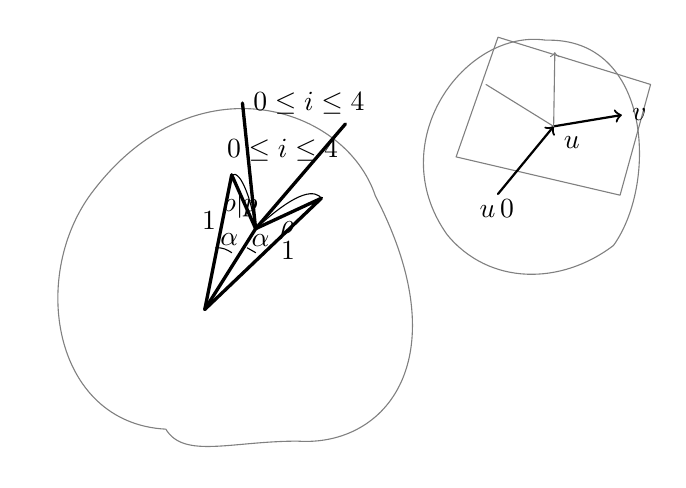
\begin{tikzpicture}[x=.76cm,y=.76cm,line cap=round,line join=round]
\draw[gray,thin] (0,0) .. controls (-1.9,.1) and (-2.3,2.6) .. (-1.2,4.0) .. controls (.5,6.2) and (3,5.4) .. (3.5,3.9) .. controls (4.9,1.2) and (3.7,-.3) .. (2.2,-.2) .. controls (1.1,-.2) and (.3,-.5) .. (0,0);
\draw[very thick] (.65,2) -- (1.5,3.35) -- (3.0,5.10);
\draw[very thick] (1.5,3.35)--(1.28,5.45) node[right] {$0\leq i\leq4$};
\draw[very thick] (.65,2)--(1.10,4.25)--(1.50,3.35)--(2.60,3.86)--cycle;
\draw (1.10,4.25) .. controls (1.26,4.35) and (1.45,3.75) .. (1.50,3.35) .. controls (2.25,4.04) and (2.5,3.98) .. (2.60,3.86);
\draw (.83,3.03) .. controls (.95,3.04) and (1.02,3) .. (1.1,2.95);
\draw (1.36,3.03)--(1.50,2.95);
\node at (.72,3.49) {$1$}; \node at (1.23,3.75) {$\unsure{\rho|p}$}; \node at (1.06,3.17) {$\alpha$};
\node at (1.58,3.16) {$\alpha$}; \node at (2.02,3.32) {$\rho$}; \node at (2.04,2.98) {$1$};
\node at (1.95,4.66) {$0\leq i\leq4$};
\draw[gray,thin] (4.7,3.25) .. controls (3.6,4.8) and (5.0,6.7) .. (6.35,6.5) .. controls (8.12,6.55) and (8.22,4.1) .. (7.48,3.07) .. controls (6.6,2.4) and (5.4,2.4) .. (4.7,3.25);
\draw[gray,thin] (4.85,4.55)--(5.55,6.55)--(8.10,5.76)--(7.59,3.91)--cycle;
\draw[->,thick] (5.55,3.93)--(6.48,5.06) node[below right] {$u$};
\draw[->,thick] (6.48,5.06)--(7.62,5.25) node[right] {$v$};
\draw[gray,->] (6.48,5.06)--(6.50,6.3);
\draw[gray] (5.35,5.76)--(6.48,5.06); \node at (5.53,3.69) {$\deleted{\unsure{u}}\,0$};
\end{tikzpicture}}
\margin{$\frac{4\pi}{5}<\frac{2\pi}{3}$\par $\frac{\pi}{3}<$}

\figure{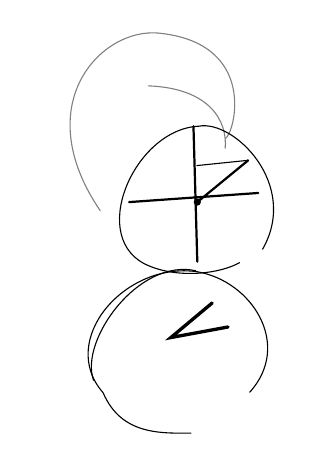
\begin{tikzpicture}[line cap=round,x=.61cm,y=.61cm]
\draw[gray] (-2.0,4.2) .. controls (-3.5,6.4) and (-2,8.0) .. (-.8,7.9) .. controls (1.3,7.7) and (.8,5.8) .. (.6,5.7);
\draw[gray] (-1.0,6.8) .. controls (.3,6.75) and (.65,6.05) .. (.6,5.5);
\draw (1.38,3.4) .. controls (2.15,4.75) and (.78,6.1) .. (.05,5.96) .. controls (-1.3,5.9) and (-2.3,3.58) .. (-.98,3.05) .. controls (-.33,2.78) and (.52,2.9) .. (.90,3.12);
\draw[thick] (.02,3.14)--(-.06,5.96) (.02,4.38)--(1.08,5.25) (-1.4,4.38)--(1.29,4.57);
\draw[thin] (.01,5.14)--(1.08,5.25); \fill (.02,4.38) circle (.075);
\draw (1.11,.42) .. controls (2.0,1.4) and (1.17,2.73) .. (.02,2.93) .. controls (-1.49,3.15) and (-2.9,1.5) .. (-1.94,.41) .. controls (-1.56,-.48) and (-.72,-.43) .. (-.11,-.43);
\draw[thin] (-2.14,.67) .. controls (-2.44,1.5) and (-1.2,3.22) .. (-.01,2.95);
\draw[very thick] (.33,2.28)--(-.53,1.56)--(.66,1.78);
\end{tikzpicture}}
\margin{$\frac{\unsure{2|1|4}\pi}{5}\unsure{>|\to}\frac{\pi}{6}\;?$ \par $\frac{4\pi}{5}\leq\frac{5\pi}{6}$}

$u,v',w'$ vecteurs unitaires
\[
 \begin{aligned}
 u&\perp v'\\
 u&\perp w'
 \end{aligned}
 \qquad v'w'=\cos\tfrac{2\pi}{5}
\]
\[
 \begin{aligned}
 x(\alpha)&=u\cos\alpha+v'\sin\alpha\\
 y(\alpha)&=u\cos\alpha+w'\sin\alpha
 \end{aligned}
\]
\[
 x(\alpha)-u=u(\cos\alpha-1)+v'\sin\alpha
\]
\[
 \begin{aligned}
 \|x(\alpha)-u\|^2&=\|y(\alpha)-u\|^2=(\cos\alpha-1)^2+\sin^2\alpha=2-2\cos\alpha\\
 &=4\sin^2\tfrac{\alpha}{2}\qquad (1-\cos\alpha=2\sin^2\tfrac{\alpha}{2}\\
 \|x(\alpha)-u\|&=2\sin\tfrac{\alpha}{2}\qquad\qquad 1-\cos^2\tfrac{\alpha}{2}+\sin^2\tfrac{\alpha}{2}
 \end{aligned}
\]
\[
 \begin{aligned}
 \|x(\alpha)-y(\alpha)\|^2&=\|v'\sin\alpha-w'\sin\alpha\|^2\\
 &=\sin^2\alpha\;\|v'-w'\|^2=\sin^2\alpha\,(2-2\cos\tfrac{2\pi}{5})\\
 &\deleted{=\sin^2\alpha+\sin^2\alpha-2\cos\tfrac{\unsure{\pi|2\pi}}5\sin^2\alpha}\\
 &=4\sin^2\alpha\sin^2\tfrac{\pi}{\unsure{5|4}}=\deleted{8\sin^2\tfrac{\alpha}{2}\sin^2\tfrac{\alpha}{2}}\;\sin\tfrac{\pi}{5}
 \end{aligned}
\]
\[
 \|x(\alpha)-y(\alpha)\|=2\sin\alpha\sin\tfrac{\pi}{5}
 =4\sin\tfrac{\alpha}{2}\cos\tfrac{\alpha}{2}\sin\tfrac{\pi}{\unsure{4|5}}
\]
\[
 \|x(\alpha)-u\|=\|y(\alpha)-u\|=\|x(\alpha)-y(\alpha)\|
\]
\[
 \Longleftrightarrow\quad 2\cos\tfrac{\alpha}{2}\sin\tfrac{\pi}{5}=1
 \qquad\text{i.e.}\quad \boxed{\cos\tfrac{\alpha}{2}=\frac{1}{2\sin{\pi/5}}}
\]
\margin{\uline{NB} \ $2\sin\frac{\pi}{5}$ = côté du pentagone régulier unité}
% archive sheet number: 17
